\documentclass[a4paper, 11pt, titlepage]{article}

% Including needed packages
\usepackage[margin=2cm]{geometry}
\usepackage{amsmath}
\usepackage{amssymb}
\usepackage{bbm}
\usepackage{dsfont}
\usepackage{graphicx}
\usepackage{subfig}
\usepackage{float}
\usepackage{biblatex}
\bibliography{report}

\newcommand{\norm}[1]{\left|\left|#1\right|\right|}
\newcommand{\argmin}{\text{argmin}}

\title
{{\em Machine learning lab course}\\
Problem set 3: Kernel Ridge Regression, Cross-validation}
\author{ROHRMANN Till, Matrnr: 343756\\
\texttt{till.rohrmann@campus.tu-berlin.de}}
\date{\today}

\begin{document}

\maketitle

\part{Introduction}
\label{part:introduction}

In the context of this problem set, I dealt with the topics of kernel ridge regression and cross-validation.
I implemented a generic cross-validation method which could also be used for other problems.
Furthermore, I realized the kernel ridge regression with the leave-one-out cross-validation (LOOCV) optimization.
I then applied the implementations on several data sets to find for each data set the best classifier.
The parameters for the kernel ridge regression method and the kernel have been estimated by the cross-validation method.
Furthermore, the behavior of a empirical ROC-curve is compared to its analytical counterpart on a toy example.

\section{Kernel ridge regression}

The ridge regression is a method to regularize ill-posed problems.
Assume we want to solve the problem
\begin{eqnarray*}
	A\mathbf{w} &=& \mathbf{b}
\end{eqnarray*}
and there exists no $\mathbf{w}$ or there exists no unique $\mathbf{w}$, then the problem is ill-posed.
A way to solve this problem, is to find a solution which minimizes the squared distances, namely ordinary least squares.

\begin{eqnarray*}
	\mathbf{w}^\star &=&\argmin_{\mathbf{w}} \norm{A\mathbf{w} - \mathbf{b}}^2_{2}
\end{eqnarray*}

In the following work, we will apply the ridge regression method to a $2$-class classification problem.
Therefore, we will set $A=X^T$ where $X\in \mathbb{R}^{d\times m}$ is the matrix containing the $m$ data points of dimension $d$ in its columns and $\mathbf{b}=Y$ with $Y\in \{-1,1\}^n$ containing the class labels of every data point.
This leads to the following problem:
\begin{eqnarray}
	\mathbf{w}^\star &=&\argmin_{\mathbf{w}} \norm{X^T\mathbf{w} - Y}^2_{2} \label{eq:ols}
\end{eqnarray}

In order to solve it, we take the gradient of equation \eqref{eq:ols} with respect to $\mathbf{w}$ and set it to $0$.
This gives us the equation
\begin{eqnarray*}
	XX^T\mathbf{w} &=& XY
\end{eqnarray*}

The matrix $XX^T$ is the empirical covariance matrix and its eigenvectors and eigenvalues define the principal components and principal values respectively.
Since high-dimensional data has often only a few large principal values and the data is often influenced by noise, we prefer solutions which take mostly large principal components into account.
This can be achieved by adding a regularization term to the equation \eqref{eq:ols} which penalizes if $\mathbf{w}$ gets too big.
Furthermore, if $XX^T$ is singular, then the regularization term makes it invertible again.
The formulation of the ridge regression problem is:
\begin{eqnarray*}
	\mathbf{w}^\star &=& \argmin_{\mathbf{w}} \norm{Y - X^T\mathbf{w}}^2_2 + C\norm{\mathbf{w}}_2^2 \label{eq:rr}
\end{eqnarray*}
with $C$ being the regularization constant.

The kernel ridge regression can now be obtained by applying the \emph{representer theorem} to set $\mathbf{w}=X\mathbf{\alpha}$ and inserting it in equation \eqref{eq:rr}.
\begin{eqnarray*}
	\mathbf{\alpha}^\star &=& \argmin_{\mathbf{\alpha}} \norm{Y - X^TX\mathbf{\alpha}}^2_2 + C\norm{\mathbf{X\alpha}}_2^2
\end{eqnarray*}

Assuming the data points have already been transformed into feature space, that is to say $X=\left[\phi(x_1),\ldots,\phi(x_m)\right]$ we can set $X^TX=K$ to our kernel matrix with $K_{i,j} = k(x_i,x_j) = \left \langle \phi(x_i),\phi(x_j)\right \rangle$. This leads to

\begin{eqnarray*}
	\mathbf{\alpha}^\star &=& \argmin_{\mathbf{\alpha}} \norm{Y-K\mathbf{\alpha}}^2_2 + C \mathbf{\alpha}^TK\mathbf{\alpha}
\end{eqnarray*}

The solution of this problem is given by

\begin{eqnarray*}
	\mathbf{\alpha}^\star &=& (K+CI)^{-1}Y
\end{eqnarray*}

\section{Cross-Validation}

Cross-validation is a model validation technique which is primarily used to evaluate the accuracy of a prediction method.
For this purpose, the data is separated into $n$ parts.
For each of these $n$ parts the other $n-1$ parts will be used for the training and the remaining part will be used as the testing data set.
The prediction error is then averaged over all $n$ parts and considered to be a good approximation of the real prediction error.
The method can be used if one needs data from the same distribution as the training data and if it is very costly or impossible to sample new data.

Using the example of classification, we use as an error function the expected ratio of misclassification of an classifier $f$.

\begin{eqnarray*}
	err &=& \mathbb{E}\left(\mathds{1}_{f(X) \not = Y}\right)
\end{eqnarray*}

This can be approximated by the empirical expectation which has the following form.

\begin{eqnarray*}
	err_{emp} &=& \frac{1}{n} \sum_{i=1}^n \mathds{1}_{f(X_i) \not = Y_i}
\end{eqnarray*}

There we can clearly see that we need data drawn from the original data distribution.
If we don't have an explicit testing data set, then we have to apply cross-validation to calculate the classification error.


\part{Implementation}
\label{part:implementation}

\section*{Assignment 1: Cross-validation}

The implementation of the \texttt{cv} method was straight forward and I basically implemented the version from the handbook.
What it does is the following:
First it iterates over all possible combinations of parameter values for the Kernel ridge regression method.
Then it calculates the average error for each parameter candidate by iterating over the number of repetitions.
For each repetition, the data is shuffled and separated into the $n$ folds.
Then for each fold, the other $n-1$ folds are used to train the regression method and the remaining fold is used to measure its accuracy.
This accuracy measure is then summed up and the average of it is returned.
Within the context of the implementation of \texttt{cv}, I did not encounter any serious problems.
The details of the implementation can be found in file \texttt{ps3\_implementation.py}.

\section*{Assignment 2: Kernel ridge regression}

The Kernel ridge regression is encapsulated by the method $\texttt{krr}$.
I implemented it according to the specification found in the handbook.
This holds true for the usual kernel ridge regression method as well as for the efficient leave-one-out cross-validation.
Leave-one-out cross-validation allows to efficiently estimate the regularization constant $C$ by performing implicitly a $m$ fold cross-validation without having to invert each time the regularized kernel matrix.
The error of the LOOCV is given by:
\begin{eqnarray}
	err &=& \frac{1}{n}\sum_{i=1}^n\left(\frac{Y_i - (K(K+CI)^{-1}Y)_i}{1-(K(K+CI)^{-1})_{ii}} \right)^2 \label{eq:LOOCV}
\end{eqnarray}
The only difficulty I encountered while implementing the kernel ridge regression method was the proper choice of the interval of $C$.
Since the kernel matrices for the polynomial kernel of high degree become quickly ill-conditioned, one cannot use a fixed range for $C$ because the regularization constant has to be higher the worse the condition number of the kernel matrix is.
In fact, it has to compensate for the bad condition so that the regularized matrix is invertible again.
Therefore I set the range to be dynamically chosen depending on the eigenvalues of the kernel matrix.
In fact the logarithmic interval between the minimal and maximal eigenvalue was chosen.
For the case that the kernel matrix is singular and has $0$ valued eigenvalues I bounded the interval from below by a minimal value $\epsilon=10^{-10}$.
Thus, the $C$ is logarithmically chosen from the interval
\begin{eqnarray*}
	C &\in& [\max(\min(eigenvalues(K),\epsilon)), \max(eigenvalues(K)) ]
\end{eqnarray*}

This guarantees that the regularized matrix is at least for some $C$ invertible.
Another problem arises if the matrix $K(K+CI)^{-1}$ has the value $1$ on its diagonal, because then we will divide by $0$ in the equation \eqref{eq:LOOCV}.
This is the case if $C$ has been chosen too small.
Therefore, I check for this condition.
If the condition is true, then I discard the $C$ value and continue with the next higher value.

The problem of ill-conditioned kernel matrices holds also for the usual kernel ridge regression case where one has specified a fixed interval for the regularization constant.
This means that one has to check for a bad condition number and discard the corresponding candidate set of parameter values as not suitable.
In the implementation I chose the maximum condition number to be \texttt{1/sys.float\_info.epsilon}.

The details of the mathematical derivation can be found in the handbook and the implementation is in the file \texttt{ps3\_implementation.py}.

\part{Application}
\label{part:application}

\section*{Assignment 3: Analytical and empirical ROC-Curve}

In this assignment we were supposed to calculate the empirical and analytical ROC curve for a two class data set obeying the following distributions:
\begin{eqnarray*}
	p(Y=-1) &=& \frac{1}{2}\\
	p(Y=1) &=& \frac{1}{2} \\
	p(X\mid Y=-1) &\sim& \mathcal{N}(\mu=0,\sigma^2 =1)\\
	p(X\mid Y=1) &\sim& \mathcal{N}(\mu=2,\sigma^2=1)
\end{eqnarray*}

Furthermore, we had to use a linear classifier for this task:
\begin{eqnarray*}
	f_{x_0}(x)&=& \begin{cases}
		+1 & x > x_0\\
		-1 & x \le x_0
	\end{cases}
\end{eqnarray*}

Assuming that the class $y=1$ is the outlier class.
Since we know the distribution of the data we can analytically calculate the true positive and false positive rate respectively.

\begin{eqnarray*}
	TPR(x_0) &=& \Pr(X \le x_0 \mid y=-1)\\
		&=& \int_{-\infty}^{x_0} \frac{1}{\sqrt{2\pi}}\exp(-\frac{1}{2}x^2)\ dx\\
	FPR(x_0) &=& \Pr(X \le x_0 \mid y=1)\\
		&=& \int_{-\infty}^{x_0} \frac{1}{\sqrt{2\pi}}\exp(-\frac{1}{2}(x-2)^2)\ dx
\end{eqnarray*}

This is nothing else than the cumulative distribution function of a Gaussian distributed random variable.
Python provides us with the function \texttt{scipy.stats.norm.cdf} to easily calculate it.

The empirical ROC curve is approximated by drawing $k$ samples from the mixture distribution and then simply counting those which have been correctly classified for the class $Y=-1$ and wrongly classified for the class $Y=1$.

\begin{eqnarray*}
	TPR_{emp}(x_0) &=& \frac{\sum_{i=1}^k \mathds{1}_{Y_i=-1}\cdot \mathds{1}_{X_i \le x_0}}{\sum_{i=1}^k \mathds{1}_{Y_i = -1}}\\
	FPR_{emp}(x_0) &=& \frac{\sum_{i=1}^k \mathds{1}_{Y_i=1}\cdot \mathds{1}_{X_i \le x_0}}{\sum_{i=1}^k \mathds{1}_{Y_i = 1}}
\end{eqnarray*}

The results can be seen in figure \ref{fig:rocCurves}.
We can clearly see that the empirical ROC curve converges to the analytical ROC curve with an increasing $k$.
This is not surprisingly, because the higher the sample size is, the better is the underlying mixture distribution approximated.

\begin{figure}
	\centering
	\subfloat[\label{fig:sub:n25}]{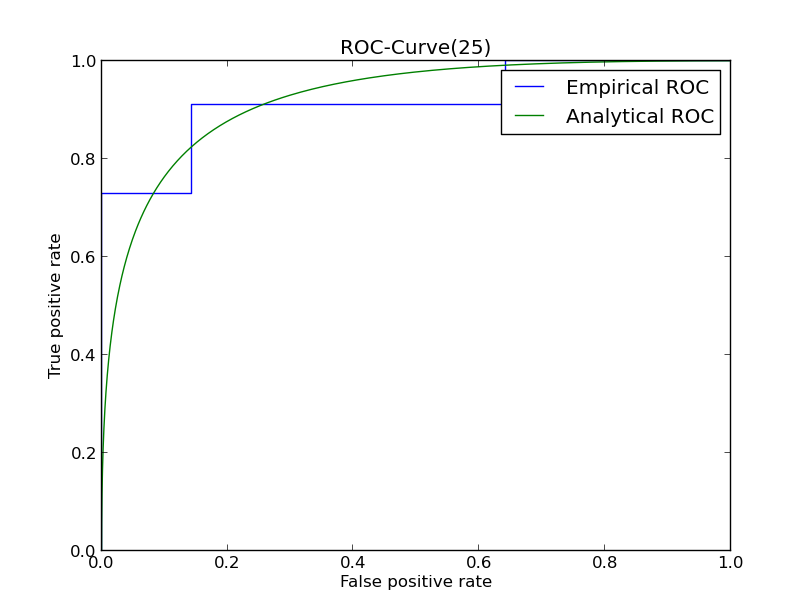
\includegraphics[width=8.5cm]{images/roc25.png}}
	\subfloat[\label{fig:sub:n50}]{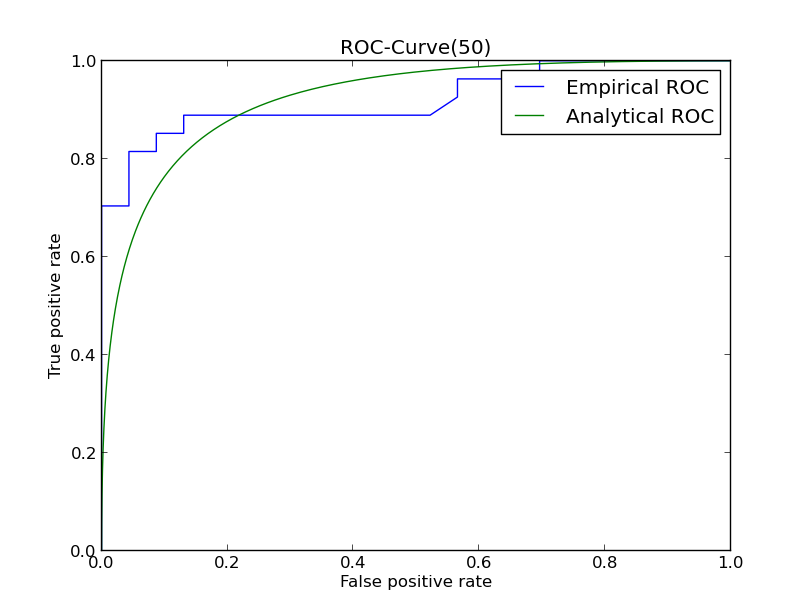
\includegraphics[width=8.5cm]{images/roc50.png}}\\
	\subfloat[\label{fig:sub:n100}]{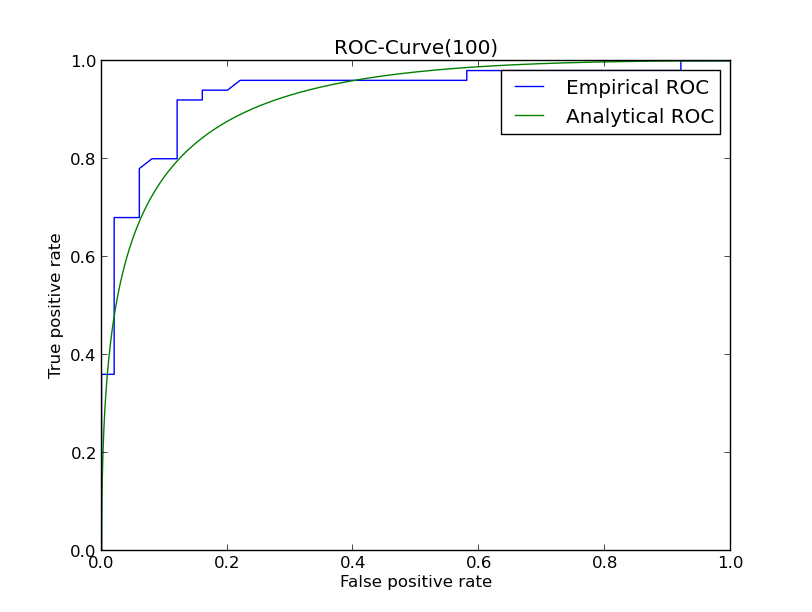
\includegraphics[width=8.5cm]{images/roc100.png}}
	\subfloat[\label{fig:sub:n500}]{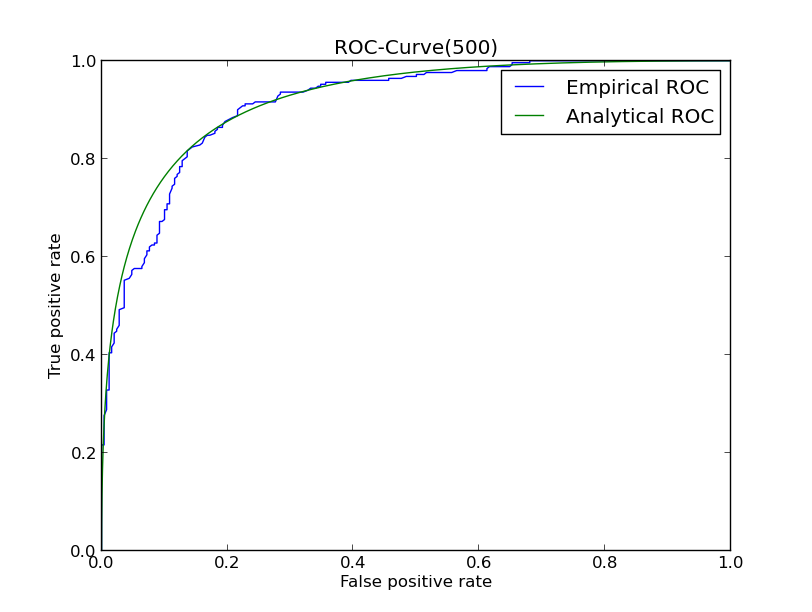
\includegraphics[width=8.5cm]{images/roc500.png}}\\
	\subfloat[\label{fig:sub:n1000}]{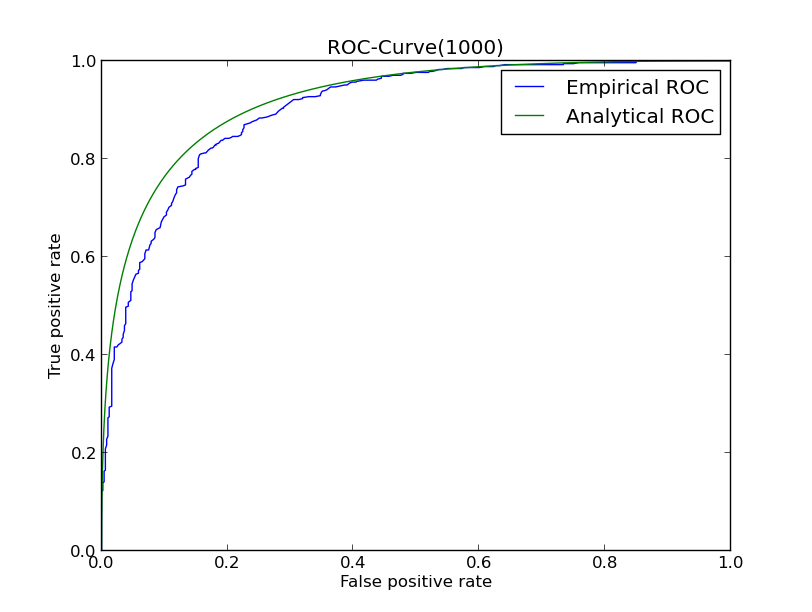
\includegraphics[width=8.5cm]{images/roc1000.png}}
	\subfloat[\label{fig:sub:n10000}]{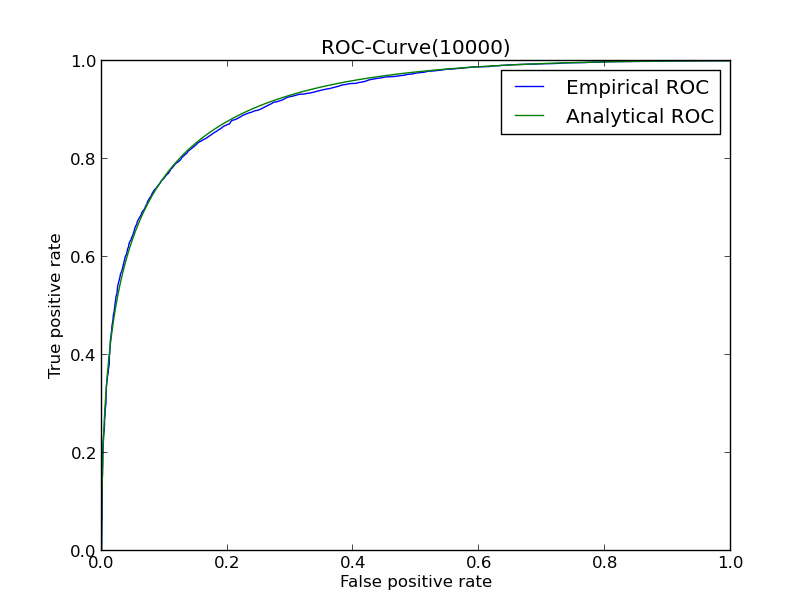
\includegraphics[width=8.5cm]{images/roc10000.png}}
	\caption{ROC curves for different sampling sizes: \protect\subref{fig:sub:n25} $k=25$, \protect\subref{fig:sub:n50} $k=50$, \protect\subref{fig:sub:n100} $k=100$, \protect\subref{fig:sub:n500} $k=500$, \protect\subref{fig:sub:n1000} $k=1000$ and \protect\subref{fig:sub:n10000} $k=10000$.}
	\label{fig:rocCurves}
\end{figure}

\section*{Assignment 4: Data set classification}

In this assignment we were supposed to apply the \texttt{cv} and the \texttt{krr} method on several data sets which are usually used in machine learning for benchmarking classification algorithms.
The data sets with their dimensionalities and sample size are shown in table \ref{tab:datasets}.
For each data set a classifier was estimated using the \texttt{cv} method without and with LOOCV.
There are $3$ different kernels supported, namely the linear, polynomial and the Gaussian kernel.
For all cross-validations the number of folds was set to $\texttt{nfolds}=10$ and the number of repetitions was set to $\texttt{nrepetitions}=5$.
For each of these kernels the best parameters were calculated by cross-validation.
The intervals for the kernel parameter values used by the cross-validation for all data sets can be seen in table \ref{tab:parametervalues}.
The difference between the cross-validation using the kernel ridge regression with LOOCV is that the regularization interval is set to $[0]$.
Then the best of the three kernels, namely the one with the lowest \texttt{cvloss} value, was chosen as the best classifier for each data set.

The results of the cross-validation without using KRR with LOOCV are shown in table \ref{tab:results} and the ones using KRR with LOOCV are shown in table \ref{tab:resultsLOOCV}.
The plots of the ROC curves of the different data sets can be found in figures \ref{fig:image}, \ref{fig:ringnorm}, \ref{fig:flaresolar}, \ref{fig:banana} and \ref{fig:diabetes}.
We can clearly see that there are some data sets which can be well classified with the tested kernels such as \texttt{image}, \texttt{ringnorm} and \texttt{banana} whereas \texttt{diabetes} and \texttt{flare-solar} are much more difficult and thus the \texttt{cvloss} value is much higher.

In order to argue that the found classifiers are quite good and the choice of the value intervals was right, one can observe that the found values don't lie at the borders of the value intervals.
Furthermore, table \ref{tab:refs} compares reference classification errors using KRR for the data sets taken from a presentation held by Prof. M\"uller \cite{Mueller13} in the context of his lecture Machine Learning 2 with the obtained results.
There we can see that the results are in good accordance with the reference results, indicating that the found classifiers cannot be much improved by choosing a different set of parameters.

\setcounter{section}{4}

\subsection{ROC curves and relation between classification error and AUC}

The classification performance can also be observed in the ROC curves and the AUC values, where the easy to classify data sets have a high AUC value and the hard to classify data sets have a low AUC value.
Furthermore, one can see that a low \texttt{cvloss} value is correlated to a high AUC value and vice versa.
However, it is not the case that if the \texttt{cvloss} value of one data set is lower than the \texttt{cvloss} value of another one, that the AUC value of this data set is necessarily higher than the AUC of the other data set.

\subsection{LOOCV and normal cross-validation}

The advantage of the efficient cross-validation of the regularization compared to using \texttt{cv} to optimize \texttt{regularization} is that we have to calculate only once an eigenvalue decomposition of the kernel matrix.
Afterwards we can quite easily execute the cross validation for all regularization values without having to calculate an matrix inverse or another decomposition.
In contrast, when using \texttt{cv} we have to calculate for each regularization value a matrix inverse.
Thus, we can assume that the efficient cross-validation has a better runtime performance.

Table \ref{tab:runtime} shows the runtimes of both versions for every data set and the corresponding speed up factor.
We can clearly see that the efficient cross-validation speeds the method tremendously up.
The general speed-up lies between $6$ and $12$.
The speed-up of $33$ for the data set \texttt{flare-solar} can be explained by the fact that the LOOCV version has found the linear kernel to be the best in contrast to the normal version which found a polynomial kernel to be best.
Since the linear kernel has fewer kernel parameter than the polynomial kernel, the speed-up is even greater.
For the other data sets, the best found kernel was for both methods the same.

However, runtime is only one aspect of a classification algorithm.
What about the achieved accuracy of the prediction?
Since the efficient cross-validation for the regularization utilizes another error measure for the regularization term, it might be the case that the accuracies are different.
The LOOCV variant uses the squared distance to the true label set as an error measure instead of the zero-one-loss function.
If we compare the classification accuracies (cv loss) in the table \ref{tab:refs}, we can observe that the accuracies of the efficient cross-validation are slightly worse than those obtained with normal cross-validation.
I assume that this is due to the different error measure.

\begin{table}
	\centering
	\begin{tabular}{lll}
		Data set & Dimensionality & Sample size\\
		\hline
		image&18&1300\\
		ringnorm &20&400\\
		flare-solar &9&666\\
		banana &2& 400\\
		diabetes &8&468
	\end{tabular}
	\caption{Data sets used for the evaluation.}
	\label{tab:datasets}
\end{table}

\begin{table}
	\centering
	\begin{tabular}{lll}
		Kernel & Kernel parameter & Regularization\\
		\hline
		linear & $[0]$ & \texttt{np.logspace(-2,2,10)} \\
		polynomial & \texttt{np.arange(1,10)} & \texttt{np.logspace(-2,2,10)}\\
		gaussian & \texttt{np.logspace(-2,2,10)} & \texttt{np.logspace(-2,2,10)}
	\end{tabular}
	\caption{Kernel parameter values and regularization values used for the different kernels. For the case of KRR with LOOCV the regularization is set to $[0]$.}
	\label{tab:parametervalues}
\end{table}

\begin{table}
	\centering
	\begin{tabular}{llllll}
	Data set& cv loss & AUC & Kernel & Kernel parameter& Regularization\\
	\hline
	image & $0.0225$ & $0.998$ & Gaussian & $1.6681$& $0.0278$\\
	ringnorm & $0.0395$& $0.999$ &Gaussian & $4.6416$& $0.0774$\\
	flare-solar & $0.3499$& $0.7$& polynomial& $1$ & $0.01$\\
	banana & $0.0985$& $0.952$& Gaussian & $0.2154$ & $1.6681$\\
	diabetes & $0.2385$ & $0.805$ & Gaussian& $4.6416$& $1.6681$
	\end{tabular}
	\caption{Results of the cross validation procedure for each data set. cv loss is the average misclassification ratio of the classifier.}
	\label{tab:results}
\end{table}

\begin{table}
	\centering
	\begin{tabular}{llllll}
	Data set& cv loss& AUC & Kernel & Kernel parameter& Regularization\\
	\hline
	image & $0.0283$& $0.996$ & Gaussian & $0.5995$& $0.4043$\\
	ringnorm & $0.0475$& $0.956$ & Gaussian & $0.0774$& $1.0$\\
	flare-solar & $0.3505$& $0.695$& linear&  & $3.7391$\\
	banana & $0.106$& $0.959$ & Gaussian & $0.5995$ & $0.8431$\\
	diabetes & $0.2431$ &  $0.805$ & Gaussian& $4.6416$& $1.8293$
	\end{tabular}
	\caption{Results of the cross validation procedure using KRR with LOOCV for each data set. cv loss is the average misclassification ratio of the classifier.}
	\label{tab:resultsLOOCV}
\end{table}

\begin{table}
	\centering
	\begin{tabular}{llll}
		Data set & cv loss & cv loss LOOCV & reference loss\\
		\hline
		image & $0.0225$ & $0.0283$ & $0.028$\\
		ringnorm & $0.0395$ & $0.0475$ & $0.047$ \\
		flare-solar & $0.3499$ & $0.3505$ & $0.341$\\
		banana & $0.0985$ & $0.106$ & $0.106$ \\
		diabetes & $0.2385$ & $0.2431$ & $0.232$
	\end{tabular}
	\caption{Comparing the cv loss values obtained by the implemented algorithms with reference values from \cite{Mueller13}.}
	\label{tab:refs}
\end{table}

\begin{table}
	\centering
	\begin{tabular}{llll}
	Data set & \texttt{cv} in s & \texttt{cv} with LOOCV in s & speed-up\\
	\hline
	image & $46504$ & $3920$ & $11.9$\\
	ringnorm & $1237$ & $185$ & $6.7$\\
	flare-solar & $1843$ & $56$ & $33$ \\
	banana & $980$ & $166$ & $6$\\
	diabetes & $2284$ & $285$ & $8$
	\end{tabular}
	\caption{Runtime of efficient cross-validation with LOOCV for the regularization and normal cross-validation for the regularization for all data sets.}
	\label{tab:runtime}
\end{table}	

\begin{figure}
	\centering
	\subfloat[\label{fig:sub:image}]{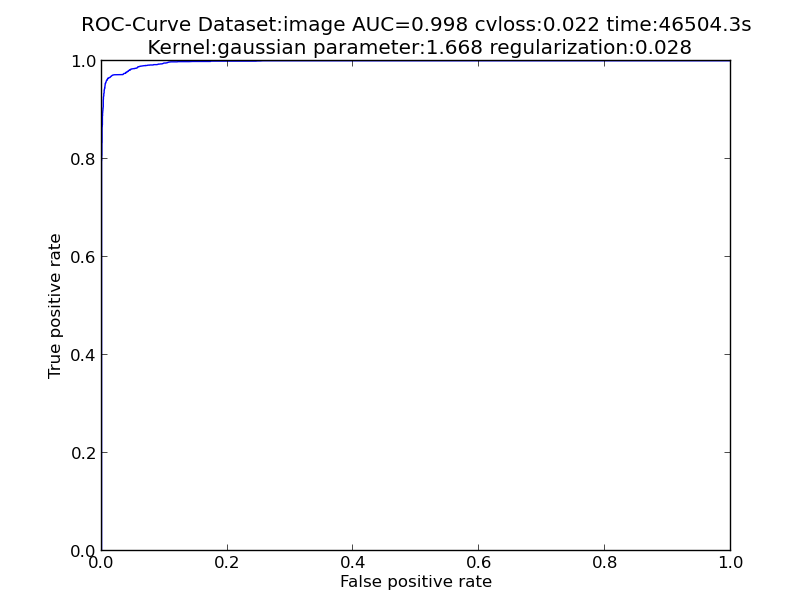
\includegraphics[width=8.5cm]{images/image.png}}
	\subfloat[\label{fig:sub:imageLOOCV}]{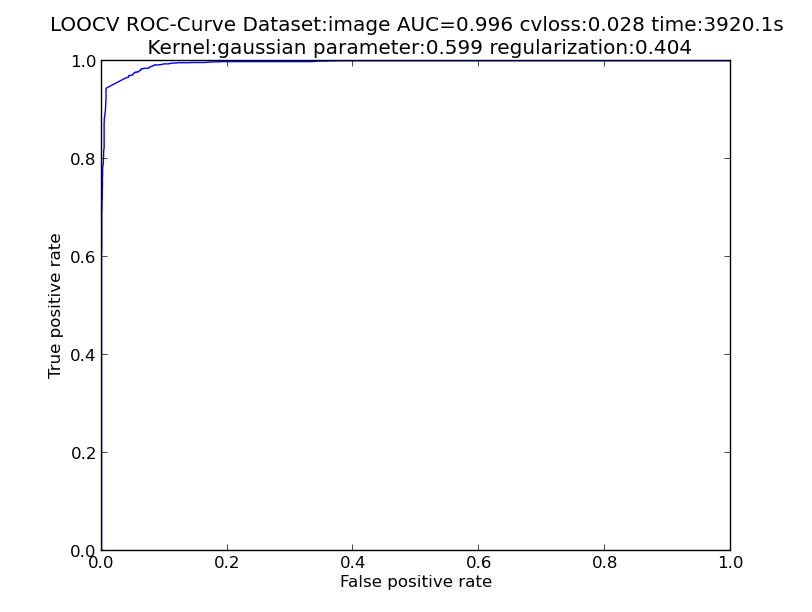
\includegraphics[width=8.5cm]{images/imageLOOCV.png}}
	\caption{ROC curves for the \texttt{image} data set. \protect\subref{fig:sub:image} normal kernel ridge regression and \protect\subref{fig:sub:imageLOOCV} kernel ridge regression with LOOCV.}
	\label{fig:image}
\end{figure}

\begin{figure}
	\centering
	\subfloat[\label{fig:sub:ringnorm}]{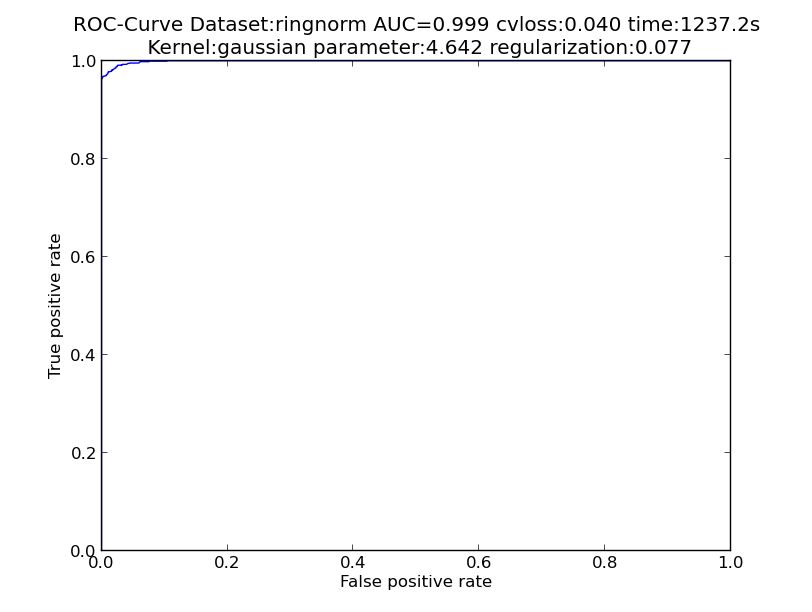
\includegraphics[width=8.5cm]{images/ringnorm.png}}
	\subfloat[\label{fig:sub:ringnormLOOCV}]{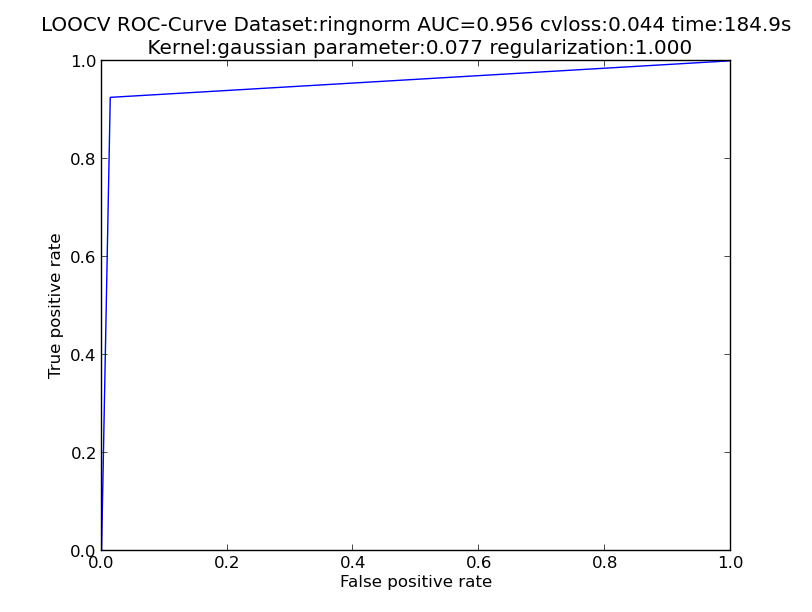
\includegraphics[width=8.5cm]{images/ringnormLOOCV.png}}
	\caption{ROC curves for the \texttt{ringnorm} data set. \protect\subref{fig:sub:ringnorm} normal kernel ridge regression and \protect\subref{fig:sub:ringnormLOOCV} kernel ridge regression with LOOCV.}
	\label{fig:ringnorm}
\end{figure}

\begin{figure}
	\centering
	\subfloat[\label{fig:sub:flaresolar}]{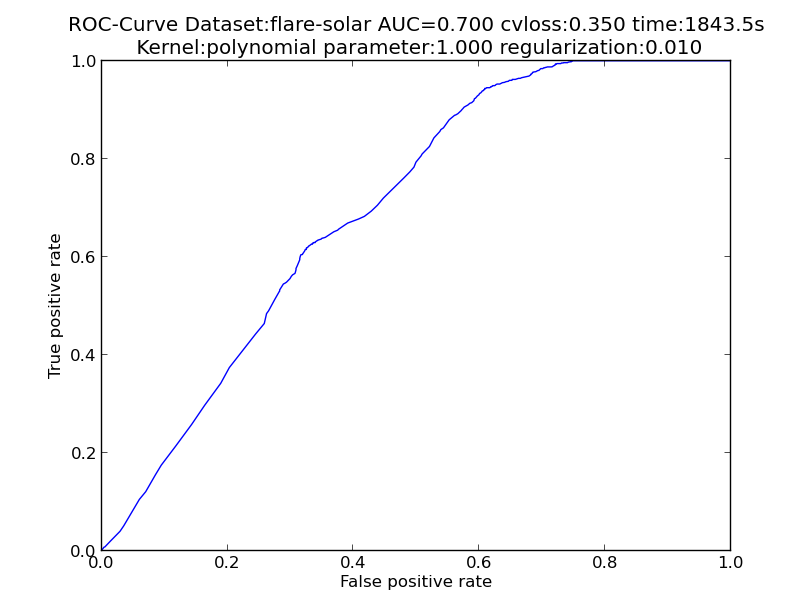
\includegraphics[width=8.5cm]{images/flaresolar.png}}
	\subfloat[\label{fig:sub:flaresolarLOOCV}]{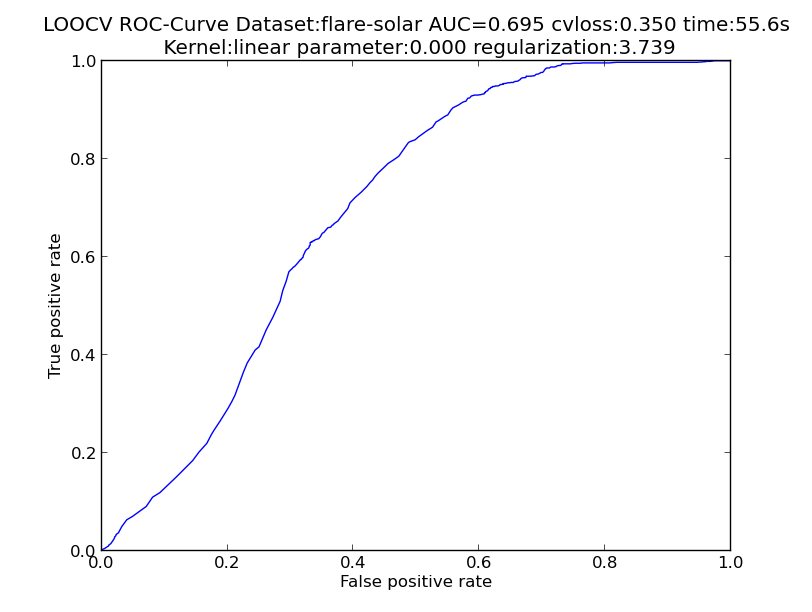
\includegraphics[width=8.5cm]{images/flaresolarLOOCV.png}}
	\caption{ROC curves for the \texttt{flare-solar} data set. \protect\subref{fig:sub:flaresolar} normal kernel ridge regression and \protect\subref{fig:sub:flaresolarLOOCV} kernel ridge regression with LOOCV.}
	\label{fig:flaresolar}
\end{figure}

\begin{figure}
	\centering
	\subfloat[\label{fig:sub:banana}]{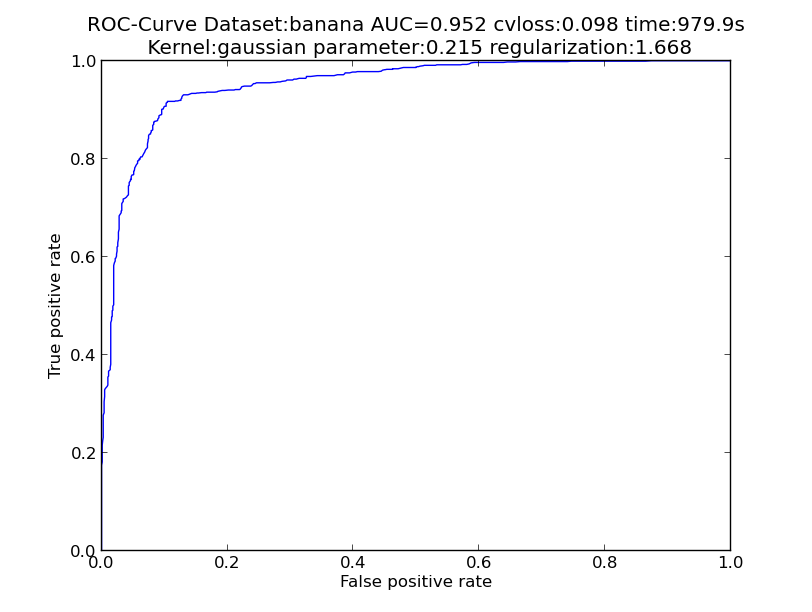
\includegraphics[width=8.5cm]{images/banana.png}}
	\subfloat[\label{fig:sub:bananaLOOCV}]{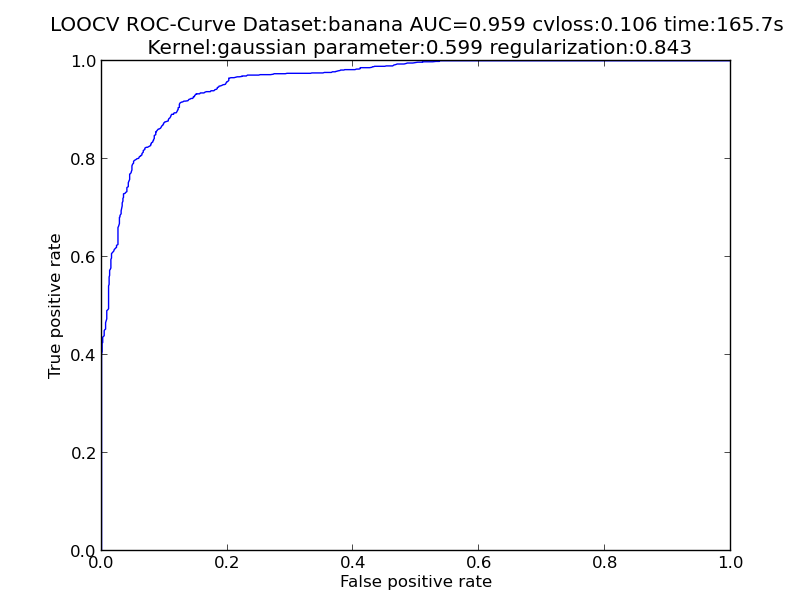
\includegraphics[width=8.5cm]{images/bananaLOOCV.png}}
	\caption{ROC curves for the \texttt{banana} data set. \protect\subref{fig:sub:banana} normal kernel ridge regression and \protect\subref{fig:sub:bananaLOOCV} kernel ridge regression with LOOCV.}
	\label{fig:banana}
\end{figure}


\begin{figure}
	\centering
	\subfloat[\label{fig:sub:diabetis}]{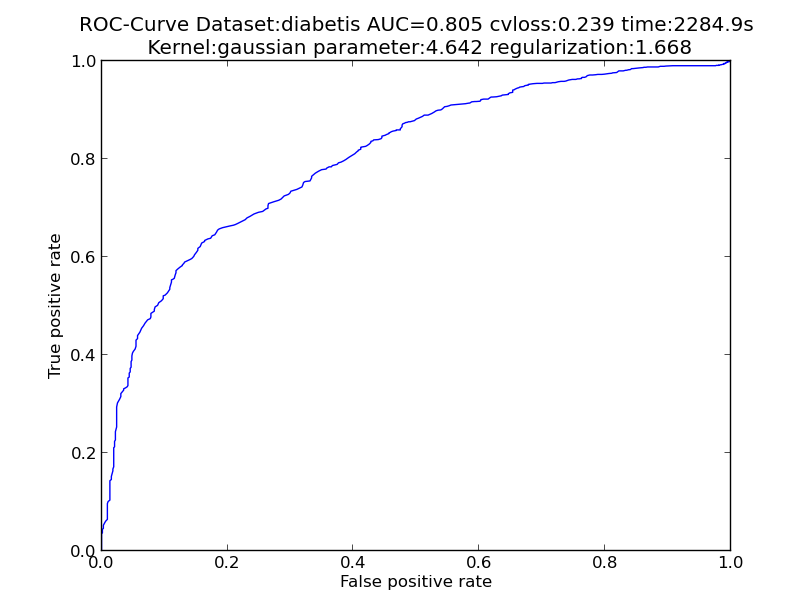
\includegraphics[width=8.5cm]{images/diabetis.png}}
	\subfloat[\label{fig:sub:diabetisLOOCV}]{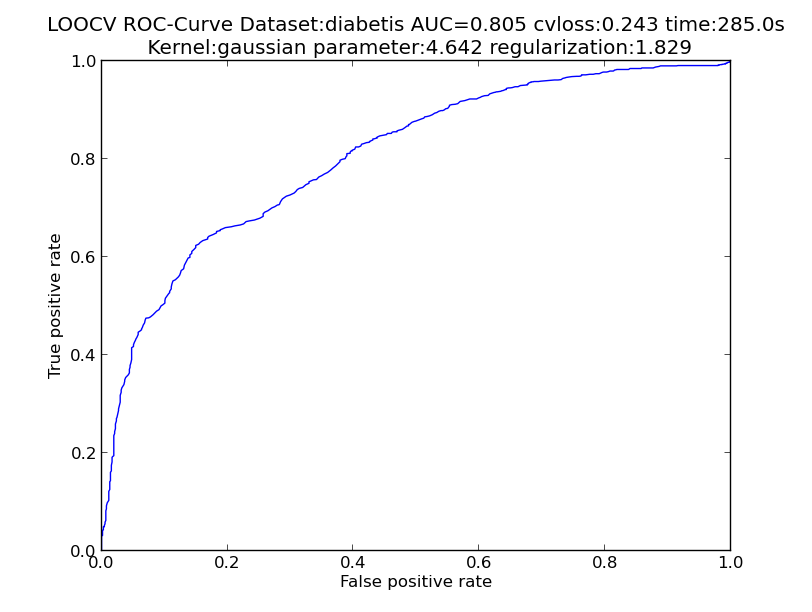
\includegraphics[width=8.5cm]{images/diabetisLOOCV.png}}
	\caption{ROC curves for the \texttt{diabetes} data set. \protect\subref{fig:sub:diabetis} normal kernel ridge regression and \protect\subref{fig:sub:diabetisLOOCV} kernel ridge regression with LOOCV.}
	\label{fig:diabetes}
\end{figure}

\printbibliography

\end{document}
